\chapter[Systems dynamics]{Systems Dynamics}

% Introduction
\chapterinitial{I}{n} many situations systems are dynamical, in that the state
or population of a number of entities or classes change according the current
state or population of the system. For example population dynamics, chemical
reactions, and systems of macroeconomics. It is often useful to be able to
predict how these systems will behave over time, though the rules that govern
these changes may be complex, and are not necessarily solvable analytically. In
these cases numerical methods and visualisation may be used, which is the focus
of this chapter.

\section{Problem}\label{sec:problem}
Consider the following scenario, where a population of 3000 people are
susceptible to infection by some disease. This population can be described by
the following parameters:

\begin{itemize}
  \item They have a birth rate $b$ of 0.01 per day;
  \item They have a death rate $d$ of 0.01 per day;
  \item For every infectious individual, the infection rate $\alpha$ is 0.3 per
  day;
  \item Infectious people recover naturally (and thus gain an immunity from the
  disease), at a recovery rate $r$ of 0.02 per day;
  \item For each day an individual is infected, they must take medication which
  costs a public healthcare system $\pounds 10$ per day.
\end{itemize}

A vaccine is produced, that allows new born individuals to gain an immunity.
This vaccine costs the public health care system a one-off cost of
$\pounds 220$ per vaccine. The healthcare providers would like to know if
achieving a vaccination rate $v$ of $85\%$ would be beneficial financially.

\section{Theory}\label{sec:theory}
% Setup - diagram & equations
The above scenario is called a compartmental model of disease, and can be shown
in the stock and flow diagram in Figure~\ref{fig:stockflow}.

\begin{figure}
\begin{center}
\includestandalone[width=\textwidth]{./assets/stock_flow_diagram}
\caption{Diagrammatic representation of the epidemiology model}
\label{fig:stockflow}
\end{center}
\end{figure}

The system has three `stocks' of different types of individuals, those
susceptible to disease ($S$), those infected with the disease ($I$), and those
who have recovered from the disease and so have gained immunity ($R$). The
levels on these stocks change according to the flows in, out, and between them,
controlled by `taps'. The amount of flow the taps let through are influenced in
a multiplicative way (either negatively or positively), by other factors, such
as external parameters (e.g. birth rate, infection rate) and the stock levels.

In this system the following taps exist, influenced by the following parameters:

\begin{itemize}
  \item \textit{external $\rightarrow S$:} Influenced positively by the birth
  rate, and negatively by the vaccine rate.
  \item \textit{$S \rightarrow I$:} Influenced positively by the infection rate,
  and the number of infected individuals.
  \item \textit{$S \rightarrow$ external:} Influenced positively by the death
  rate.
  \item \textit{$I \rightarrow R$:} Influenced positively by the recovery rate.
  \item \textit{$I \rightarrow$ external:} Influenced positively by the death
  rate.
  \item \textit{$R \rightarrow$ external:} Influenced positively by the birth
  rate and the vaccine rate.
  \item \textit{external $\rightarrow R$:} Influenced positively by the death
  rate.
\end{itemize}

Mathematically the change in stock levels are written as the derivatives, for
example the change in the number of susceptible individuals over time is denoted
by $\frac{dS}{dt}$. This is equal to the sum of the taps in or out of that
stock. Thus the system is described by the following system of differential
equations:

\begin{align}
\frac{dS}{dt} &= -\frac{\alpha SI}{N} + (1 - v)bN - dS \label{eqn:dS}\\
\frac{dI}{dt} &= \frac{\alpha SI}{N} - (r + d)I \label{eqn:dI}\\
\frac{dR}{dt} &= rI - dR + vbN \label{eqn:dR}
\end{align}

Where $N = S + I + R$ is the total number of individuals in the system.

We would like to understand the behaviour of the functions $S$, $I$ and $R$
under these rules, that is we would like to solve this system of differential
equations. This system contains some non-linear terms, implying that this may be
difficult to solve analytically, so we will use a numerical method instead.

There are a number of numerical methods, and the solvers we will use in Python
and R cleverly choose the most appropriate for the problem at hand. In general
methods for this kind of problems use the principle that the derivative denotes
the rate of instantaneous change. Thus for a differential equation
$\frac{dy}{dt} = f(t,y)$, consider the function $y$ as a discrete sequence of
points $\{y_0, y_1, y_2, y_3, \dots\}$ on
$\{t_0, t_0 + h, t_0 + 2h, t_0 + 3h, \dots\}$ then

\begin{equation}
y_{n+1} = h \times f(t_0 + nh, y_n).
\end{equation}

This sequence approaches the true solution $y$ as $h \rightarrow 0$.
Thus numerical methods, including the Runge-Kutta methods and the Euler method,
step through this sequence $\{y_n\}$, choosing appropriate values of $h$ and
employing other methods of error reduction.


\section{Solving with Python}\label{sec:solving-with-python}
In this book we will use the \mintinline{python}{odeint} method of the SciPy
library to numerically solve the above epidemiology models.

We first define the system of differential equations described in
Equations~\ref{eqn:dS}, \ref{eqn:dI} and \ref{eqn:dR}.
This is a regular Python function, where the first two arguments are the system
state and the current time respectively.

\begin{pyin}
def derivatives(y, t, vaccine_rate, birth_rate=0.01):
    """Defines the system of differential equations that
    describe the epidemiology model.

    Args:
        y: a tuple of three integers
        t: a positive float
        vaccine_rate: a positive float <= 1
        birth_rate: a positive float <= 1

    Returns:
        A tuple containing dS, dI, and dR
    """
    infection_rate = 0.3
    recovery_rate = 0.02
    death_rate = 0.01
    S, I, R = y
    N = S + I + R
    dSdt = (
        -((infection_rate * S * I) / N)
        + ((1 - vaccine_rate) * birth_rate * N)
        - (death_rate * S)
    )
    dIdt = (
        ((infection_rate * S * I) / N)
        - (recovery_rate * I)
        - (death_rate * I)
    )
    dRdt = (
        (recovery_rate * I)
        - (death_rate * R)
        + (vaccine_rate * birth_rate * N)
    )
    return dSdt, dIdt, dRdt
\end{pyin}

Using this function returns the instantaneous rate of change for each of the
three stocks, $S$, $I$ and $R$. If we begin at time 0.0, with 4 susceptible
individuals, 1 infected individual, 0 recovered individuals, and a vaccine rate
of 50\%, then:

\begin{pyin}
print(derivatives(y=(4, 1, 0), t=0.0, vaccine_rate=0.5))
\end{pyin}

\begin{pyout}
(-0.255, 0.21, 0.045)
\end{pyout}

we would expect the number of susceptible individuals to reduce by around 0.255
per time unit, the number of infected individuals to increase by 0.21 per time
unit, and the number of recovered individuals to increase by 0.045 per time
unit. Now of course, after a tiny fraction of a time unit the stock levels will
change, and thus the rates of change will change. So we will require something
more sophisticated in order to determine the true behaviour of the system.

The following function observes the system's behaviour over some time period,
using SciPy's \mintinline{python}{odeint} to numerically solve the system of
differential equations:

\begin{pyin}
from scipy.integrate import odeint


def integrate_ode(
    derivative_function,
    t,
    y0=(2999, 1, 0),
    vaccine_rate=0.85,
    birth_rate=0.01,
):
    """Numerically solve the system of differential equations.

    Args:
        derivative_function: a function returning a tuple
                             of three floats
        t: an array of increasing positive floats
        y0: a tuple of three integers (default: (2999, 1, 0))
        vaccine_rate: a positive float <= 1 (default: 0.85)
        birth_rate: a positive float <= 1 (default: 0.01)

    Returns:
        A tuple of three arrays
    """
    results = odeint(
        derivative_function,
        y0,
        t,
        args=(vaccine_rate, birth_rate),
    )
    S, I, R = results.T
    return S, I, R
\end{pyin}

Now we can use this function to investigate the difference in behaviour between
a vaccination rate of 0\% and a vaccination rate of 85\%. Let's observe the
system for two years, that is 730 days, in time steps of 0.01 days.

Begin with a vaccine rate of 0\%:

\begin{pyin}
import numpy as np
from scipy.integrate import odeint

t = np.arange(0, 730.01, 0.01)
S, I, R = integrate_ode(derivatives, t, vaccine_rate=0.0)
\end{pyin}

Now \mintinline{python}{S}, \mintinline{python}{I} and \mintinline{python}{R}
are arrays of values of the stock levels of $S$, $I$ and $R$ over the time
steps \mintinline{python}{t}.
Using \mintinline{python}{matplotlib} we can plot these to visualise their
behaviour.
The following code gives the plot shown in Figure~\ref{fig:plot_no_vaccine}.


\begin{pyin-no-test}
import matplotlib.pyplot as plt

fig, ax = plt.subplots(1)
ax.plot(t, S, label='Susceptible')
ax.plot(t, I, label='Infected')
ax.plot(t, R, label='Recovered')
ax.legend(fontsize=12)
fig.savefig("plot_no_vaccine_python.pdf")
\end{pyin-no-test}


\begin{figure}
\begin{center}
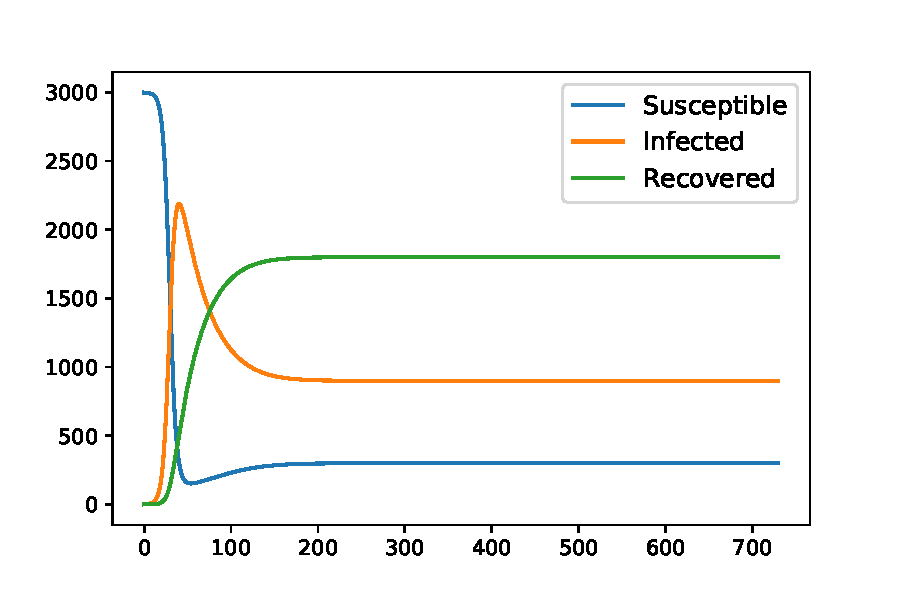
\includegraphics[width=0.6\textwidth]{./assets/plot_no_vaccine_python.pdf}
\end{center}
\caption{Output of code line 737-742}
\label{fig:plot_no_vaccine}
\end{figure}

We observe that the number of infected individuals increases quickly, and in
fact the rate of change increases as more individuals are infected. However
this growth slows down as there are fewer susceptible individuals to infect. Due
to the equal birth and death rates the overall population size remains constant;
but we also see after some time period (around 300 time units) the levels of
susceptible, infected, and recovered individuals becomes seemingly steady, and
the disease becomes endemic. We can estimate once this steadiness occurs, around
10\% of the population remain susceptible to the disease, 30\% are infected, and
60\% are recovered and immune.

Now with a vaccine rate of 85\%:

\begin{pyin}
t = np.arange(0, 730.01, 0.01)
S, I, R = integrate_ode(derivatives, t, vaccine_rate=0.85)
\end{pyin}

And again we can plot these to visualise their behaviour. The following code
gives the plot shown in Figure~\ref{fig:plot_with_vaccine}.

\begin{pyin-no-test}
fig, ax = plt.subplots(1)
ax.plot(t, S, label='Susceptible')
ax.plot(t, I, label='Infected')
ax.plot(t, R, label='Recovered')
ax.legend(fontsize=12)
fig.savefig("plot_with_vaccine_python.pdf")
\end{pyin-no-test}

\begin{figure}
\begin{center}
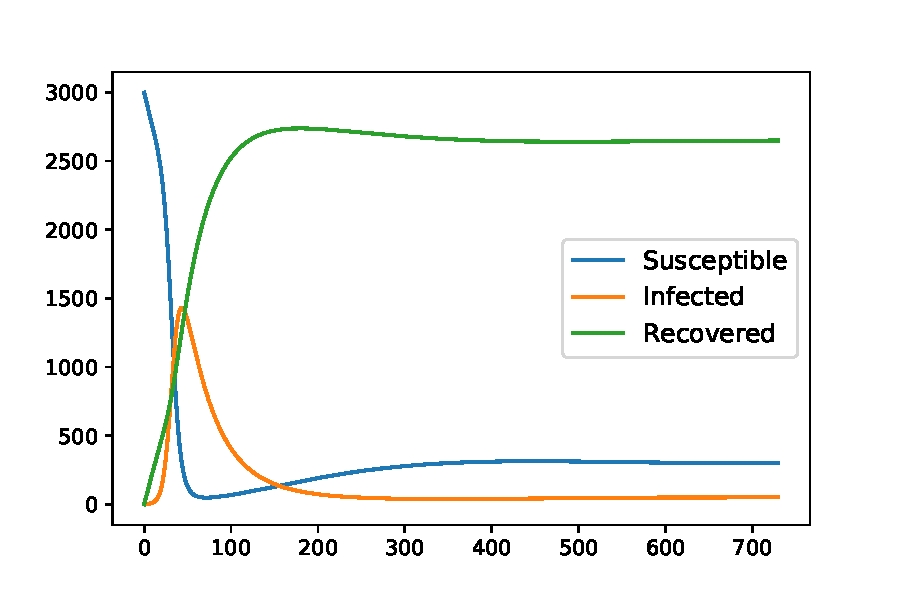
\includegraphics[width=0.6\textwidth]{./assets/plot_with_vaccine_python.pdf}
\end{center}
\caption{Output of code line 745-750}
\label{fig:plot_with_vaccine}
\end{figure}

With vaccination the disease remains endemic, however now we estimate that once,
steadiness occurs, around 10\% of the population remain susceptible to the
disease, 1.7\% are infected, and 88.3\% are immune or recovered and immune.

We've seen that vaccination lowers the percentage of the population living with
the infection, which will lower the public healthcare system's medication costs.
Let's now investigate if this saving is comparable to the cost of providing the
vaccination to the newborns.

The following function calculates the total cost to the public healthcare
system, that is the sum of the medication costs for those living with the
infection and the vaccination costs:

\begin{pyin}
def daily_cost(
    derivative_function=derivatives, vaccine_rate=0.85
):
    """Calculates the daily cost to the public health system
    after 2 years.

    Args:
        derivative_function: a function returning a tuple
                             of three floats
        vaccine_rate: a positive float <= 1 (default: 0.85)

    Returns:
        the daily cost
    """
    max_time = 730
    time_step = 0.01
    birth_rate = 0.01
    vaccine_cost = 220
    medication_cost = 10
    t = np.arange(0, max_time + time_step, time_step)
    S, I, R = integrate_ode(
        derivatives,
        t,
        vaccine_rate=vaccine_rate,
        birth_rate=birth_rate,
    )
    N = S[-1] + I[-1] + R[-1]
    daily_vaccine_cost = (
        N * birth_rate * vaccine_rate * vaccine_cost
    ) / time_step
    daily_meds_cost = (I[-1] * medication_cost) / time_step
    return daily_vaccine_cost + daily_meds_cost
\end{pyin}

Now let's compare the total daily cost with and without vaccination. Without
vaccinations:

\begin{pyin}
cost = daily_cost(vaccine_rate=0.0)
print(round(cost, 2))
\end{pyin}

which gives

\begin{pyout}
900000.0
\end{pyout}

Therefore without vaccinations, once the infection is endemic, the public health
care system would expect to spend $\pounds 900,000$ a day.

With a vaccine rate of 85\%:

\begin{pyin}
cost = daily_cost(vaccine_rate=0.85)
print(round(cost, 2))
\end{pyin}

which gives

\begin{pyout}
611903.36
\end{pyout}

So vaccinating 85\% of newborns would cost the public health care system, once
the infection is endemic $\pounds 611,903.36$ a day. That is a saving of around
32\%.





\section{Solving with R}\label{sec:solving-with-R}
In this book we will use the \mintinline{R}{deSolve} library to numerically
solve the above epidemiology models.

We first define the system of differential equations described in
Equations~\ref{eqn:dS}, \ref{eqn:dI} and \ref{eqn:dR}. This is an R function
where the arguments are the current time, the system state, and a list of other
parameters, respectively.

\begin{Rin}
#' Defines the system of differential equations that describe
#' the epidemiology model.
#'
#' @param t a positive float
#' @param y a tuple of three integers
#' @param vaccine_rate a positive float <= 1
#' @param birth_rate a positive float <= 1
#'
#' @return a list containing dS, dI, and dR
derivatives <- function(t, y, parameters){
  infection_rate <- 0.3
  recovery_rate <- 0.02
  death_rate <- 0.01
  with(as.list(c(y, parameters)), {
    N <- S + I + R
    dSdt <- ( - ( (infection_rate * S * I) / N)
             + ( (1 - vaccine_rate) * birth_rate * N)
             - (death_rate * S))
    dIdt <- ( ( (infection_rate * S * I) / N)
            - (recovery_rate * I)
            - (death_rate * I))
    dRdt <- ( (recovery_rate * I)
             - (death_rate * R)
             + (vaccine_rate * birth_rate * N))
    list(c(dSdt, dIdt, dRdt))
  })
}
\end{Rin}

Using this function returns the instantaneous rate of change for each of the
three stocks, $S$, $I$ and $R$. If we begin at time 0.0, with 4 susceptible
individuals, 1 infected individual, 0 recovered individuals, a vaccine rate
of 50\% and a birth rate of 0.01, then:

\begin{Rin}
derivatives(t = 0,
            y = c(S = 4, I = 1, R = 0),
            parameters = c(vaccine_rate = 0.5,
                           birth_rate = 0.01)
)
\end{Rin}

\begin{Rout}
[[1]]
[1] -0.255  0.210  0.045

\end{Rout}

we would expect the number of susceptible individuals to reduce by around 0.255
per time unit, the number of infected individuals to increase by 0.21 per time
unit, and the number of recovered individuals to increase by 0.045 per time
unit. Now of course, after a tiny fraction of a time unit the stock levels will
change, and thus the rates of change will change. So we will require something
more sophisticated in order to determine the true behaviour of the system.

The following function observes the system's behaviour over some time period,
using the \mintinline{R}{deSolve} library to numerically solve the system of
differential equations:

\begin{Rin}
library(deSolve)

#' Numerically solve the system of differential equations
#'
#' @param t an array of increasing positive floats
#' @param y0 list of integers (default: c(S=2999, I=1, R=0))
#' @param birth_rate a positive float <= 1 (default: 0.01)
#' @param vaccine_rate a positive float <= 1 (default: 0.85)
#'
#' @return a matrix of times, S, I and R values
integrate_ode <- function(times,
                          y0 = c(S = 2999, I = 1, R = 0),
                          birth_rate = 0.01,
                          vaccine_rate = 0.84){
  params <- c(birth_rate = birth_rate,
                  vaccine_rate = vaccine_rate)
  ode(y = y0,
      times = times,
      func = derivatives,
      parms = params)
}
\end{Rin}

Now we can use this function to investigate the difference in behaviour between
a vaccination rate of 0\% and a vaccination rate of 85\%. Let's observe the
system for two years, that is 730 days, in time steps of 0.01 days.

Begin with a vaccine rate of 0\%:

\begin{Rin}
times <- seq(0, 730, by = 0.01)
out <- integrate_ode(times, vaccine_rate = 0.0)
\end{Rin}

Now \mintinline{R}{out}, is a matrix with four columns,  \mintinline{R}{time},
\mintinline{R}{S}, \mintinline{R}{I} and \mintinline{R}{R}, which are arrays of
values of the time points, and the stock levels of $S$, $I$ and $R$ over the
time respectively.
We can plot these to visualise their behaviour.
The following code gives the plot shown in Figure~\ref{fig:plot_no_vaccine_R}.


\begin{Rin-no-test}
pdf("plot_no_vaccine_R.pdf", width = 7, height = 5)
plot(out[, "time"], out[, "S"], type = "l", col = "blue")
lines(out[, "time"], out[, "I"], type = "l", col = "orange")
lines(out[, "time"], out[, "R"], type = "l", col = "darkgreen")
dev.off()
\end{Rin-no-test}


\begin{figure}
\begin{center}
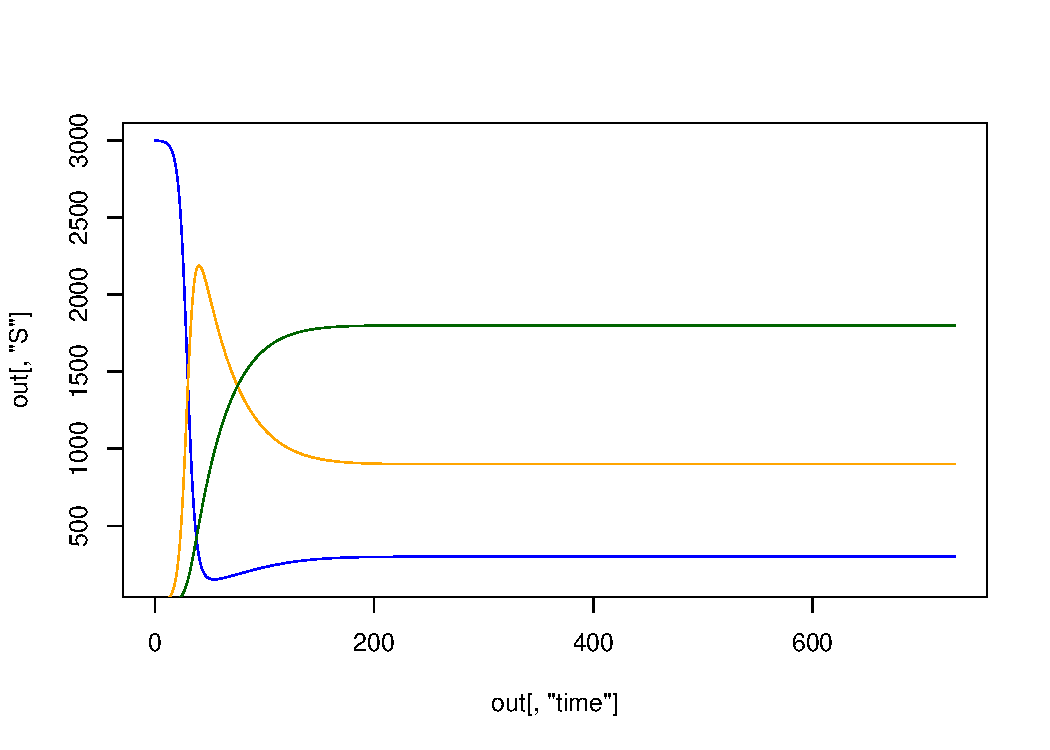
\includegraphics[width=0.6\textwidth]{./assets/plot_no_vaccine_R.pdf}
\end{center}
\caption{Output of code line 846-850}
\label{fig:plot_no_vaccine_R}
\end{figure}

We observe that the number of infected individuals increases quickly, and in
fact the rate of change increases as more individuals are infected. However
this growth slows down as there are fewer susceptible individuals to infect. Due
to the equal birth and death rates the overall population size remains constant;
but we also see after some time period (around 300 time units) the levels of
susceptible, infected, and recovered individuals becomes seemingly steady, and
the disease becomes endemic. We can estimate once this steadiness occurs, around
10\% of the population remain susceptible to the disease, 30\% are infected, and
60\% are recovered and immune.

Now with a vaccine rate of 85\%:

\begin{Rin}
times <- seq(0, 730, by = 0.01)
out <- integrate_ode(times, vaccine_rate = 0.85)
\end{Rin}

And again we can plot these to visualise their behaviour. The following code
gives the plot shown in Figure~\ref{fig:plot_with_vaccine_R}.

\begin{Rin-no-test}
pdf("plot_with_vaccine_R.pdf", width = 7, height = 5) 
plot(out[, "time"], out[, "S"], type = "l", col = "blue")
lines(out[, "time"], out[, "I"], type = "l", col = "orange")
lines(out[, "time"], out[, "R"], type = "l", col = "darkgreen")
dev.off()
\end{Rin-no-test}


\begin{figure}
\begin{center}
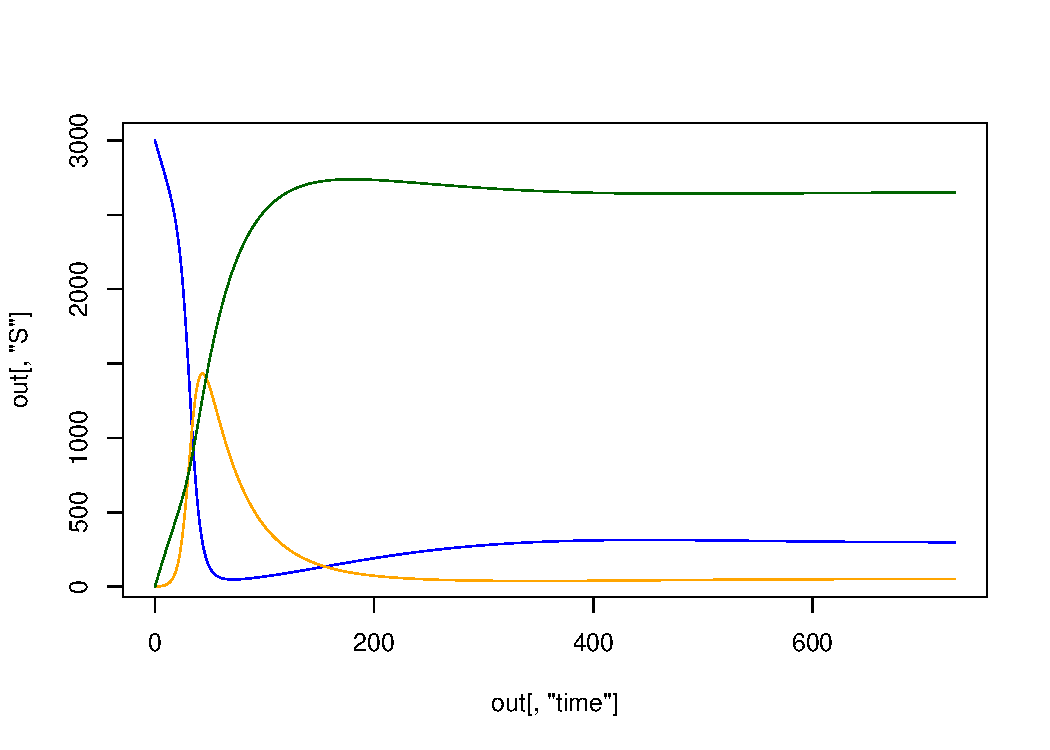
\includegraphics[width=0.6\textwidth]{./assets/plot_with_vaccine_R.pdf}
\end{center}
\caption{Output of code line 853-857}
\label{fig:plot_with_vaccine_R}
\end{figure}

With vaccination the disease remains endemic, however now we estimate that once,
steadiness occurs, around 10\% of the population remain susceptible to the
disease, 1.7\% are infected, and 88.3\% are immune or recovered and immune.

We've seen that vaccination lowers the percentage of the population living with
the infection, which will lower the public healthcare system's medication costs.
Let's now investigate if this saving is comparable to the cost of providing the
vaccination to the newborns.

The following function calculates the total cost to the public healthcare
system, that is the sum of the medication costs for those living with the
infection and the vaccination costs:

\begin{Rin}
#' Calculates the daily cost to the public health
#' system after 2 years
#'
#' @param derivative_function: a function returning a
#'                             list of three floats
#' @param vaccine_rate: a positive float <= 1 (default: 0.85)
#'
#' @return the daily cost
daily_cost <- function(derivative_function = derivatives,
                       vaccine_rate = 0.85){
  max_time <- 730
  time_step <- 0.01
  birth_rate <- 0.01
  vaccine_cost <- 220
  medication_cost <- 10
  times <- seq(0, max_time, by = time_step)
  out <- integrate_ode(times, vaccine_rate = vaccine_rate)
  N <- sum(tail(out[, c("S", "I", "R")], n = 1))
  daily_vaccine_cost <- (N
                         * birth_rate
                         * vaccine_rate
                         * vaccine_cost) / time_step
  daily_medication_cost <- ( (tail(out[, "I"], n = 1)
                             * medication_cost)) / time_step
  daily_vaccine_cost + daily_medication_cost
}
\end{Rin}

Now let's compare the total daily cost with and without vaccination. Without
vaccinations:

\begin{Rin}
cost <- daily_cost(vaccine_rate = 0.0)
print(cost)
\end{Rin}

which gives

\begin{Rout}
[1] 9e+05
\end{Rout}

Therefore without vaccinations, once the infection is endemic, the public health
care system would expect to spend $\pounds 900,000$ a day.

With a vaccine rate of 85\%:

\begin{Rin}
cost <- daily_cost(vaccine_rate = 0.85)
print(cost)
\end{Rin}

which gives

\begin{Rout}
[1] 611903.4
\end{Rout}

So vaccinating 85\% of newborns would cost the public health care system, once
the infection is endemic $\pounds 611,903.40$ a day. That is a saving of around
32\%.



\section{Research}\label{sec:research}
